% ============================================================
%  A Self-Contained Tutoring Guide to the Itô Stochastic Integral
%  MATH 60646A, HEC Montréal
%  Follows the three-layer construction: Basic → Simple → Predictable
% ============================================================
\documentclass[11pt,a4paper]{article}

% --- Packages ---
\usepackage[utf8]{inputenc}
\usepackage[T1]{fontenc}
\usepackage{amsmath, amssymb, amsthm}
\usepackage{mathtools}
\usepackage{geometry}
\usepackage{hyperref}
\usepackage{enumitem}
\usepackage{xcolor}
\usepackage{mdframed}
\usepackage{tikz}
\usepackage{pgfplots}
\pgfplotsset{compat=1.18}
\usepackage{booktabs}
\usepackage{microtype}
\usepackage{parskip}

% --- Page layout ---
\geometry{margin=2.5cm}

% --- Colours ---
\definecolor{tutorblue}{RGB}{13,71,161}
\definecolor{tutorgold}{RGB}{183,119,41}
\definecolor{tutorgreen}{RGB}{27,94,32}
\definecolor{tutorred}{RGB}{183,28,28}
\definecolor{lightblue}{RGB}{227,242,253}
\definecolor{lightgold}{RGB}{255,248,225}
\definecolor{lightgreen}{RGB}{232,245,233}
\definecolor{lightred}{RGB}{255,235,238}

% --- Theorem environments ---
\theoremstyle{definition}
\newtheorem{definition}{Definition}[section]
\newtheorem{example}{Example}[section]
\newtheorem{exercise}{Exercise}[section]

\theoremstyle{plain}
\newtheorem{theorem}{Theorem}[section]
\newtheorem{proposition}{Proposition}[section]
\newtheorem{lemma}{Lemma}[section]

\theoremstyle{remark}
\newtheorem*{remark}{Remark}
\newtheorem*{intuition}{Intuition}
\newtheorem*{warning}{Warning}

% --- Custom boxes ---
\newmdenv[
  backgroundcolor=lightblue,
  linecolor=tutorblue,
  linewidth=1.5pt,
  roundcorner=4pt,
  innerleftmargin=10pt,
  innerrightmargin=10pt,
  innertopmargin=8pt,
  innerbottommargin=8pt,
]{tutobox}

\newmdenv[
  backgroundcolor=lightgold,
  linecolor=tutorgold,
  linewidth=1.5pt,
  roundcorner=4pt,
  innerleftmargin=10pt,
  innerrightmargin=10pt,
  innertopmargin=8pt,
  innerbottommargin=8pt,
]{keyidea}

\newmdenv[
  backgroundcolor=lightgreen,
  linecolor=tutorgreen,
  linewidth=1.5pt,
  roundcorner=4pt,
  innerleftmargin=10pt,
  innerrightmargin=10pt,
  innertopmargin=8pt,
  innerbottommargin=8pt,
]{workedex}

\newmdenv[
  backgroundcolor=lightred,
  linecolor=tutorred,
  linewidth=1.5pt,
  roundcorner=4pt,
  innerleftmargin=10pt,
  innerrightmargin=10pt,
  innertopmargin=8pt,
  innerbottommargin=8pt,
]{pitfall}

% --- Notation shortcuts ---
\newcommand{\R}{\mathbb{R}}
\newcommand{\E}{\mathbb{E}}
\newcommand{\Prob}{\mathbb{P}}
\newcommand{\F}{\mathcal{F}}
\newcommand{\calL}{\mathcal{L}}
\newcommand{\calB}{\mathcal{B}}
\newcommand{\Wt}{W_t}
\newcommand{\dW}{\,dW}
\newcommand{\dt}{\,dt}
\newcommand{\abs}[1]{\left|#1\right|}
\newcommand{\norm}[1]{\left\|#1\right\|}
\newcommand{\var}{\mathrm{Var}}
\newcommand{\cov}{\mathrm{Cov}}
\DeclareMathOperator*{\esssup}{ess\,sup}

% --- Hyperref setup ---
\hypersetup{
  colorlinks=true,
  linkcolor=tutorblue,
  urlcolor=tutorblue,
  citecolor=tutorblue,
  pdftitle={A Tutoring Guide to the Itô Stochastic Integral},
  pdfauthor={MATH 60646A Supplementary Notes},
}

% ============================================================
\begin{document}
% ============================================================

\begin{center}
  {\LARGE\bfseries\color{tutorblue}
    A Tutoring Guide to the It\^{o} Stochastic Integral}\\[8pt]
  {\large\color{tutorgold}
    From Riemann Sums to the Full It\^{o} Integral}\\[6pt]
  {\normalsize Supplementary notes for MATH 60646A, HEC Montr\'eal}\\[4pt]
  {\small Building the integral in three layers: Basic $\to$ Simple $\to$ Predictable}
\end{center}

\vspace{0.5em}
\hrule height 1.5pt
\vspace{0.5em}

\begin{tutobox}
\textbf{How to use these notes.} These notes are written as if you and I are sitting together at a whiteboard. Every definition is followed immediately by a plain-English translation. Every theorem is preceded by the \emph{intuition} that makes it feel inevitable. Every formal argument is accompanied by a worked example so you can check your understanding. The goal is not to replace your course slides but to make every line of them feel obvious in hindsight.
\end{tutobox}

\tableofcontents
\newpage

% ============================================================
\section{Before We Begin: A Recap of Classical Integration}
\label{sec:classical}
% ============================================================

\subsection{Why do we integrate at all?}

Integration is, at its heart, a machine for \emph{accumulating contributions}. When you write $\int_0^T f(t)\,dt$, you are asking: ``if $f(t)$ represents the rate at which something is changing at time $t$, what is the total accumulated change over $[0,T]$?''

In physics, $\int_0^T v(t)\,dt$ gives total displacement from velocity. In finance, $\int_0^T r_t S_t\,dt$ gives the total interest earned on a position in a bond. These integrals make sense because $t$ (or some other variable like a bond price path) is \emph{smooth enough} for the accumulation to be well-defined.

Stochastic calculus breaks this comfortable assumption. The ``integrator'' will become Brownian motion, which is nowhere differentiable and has infinite variation. Classical integration theory, as you will see, completely fails to handle this. Building a new theory of integration — the Itô integral — is the central achievement of stochastic calculus.

\subsection{The Riemann integral: a reminder}

Let $f: [0,T] \to \R$ be a continuous function. To define $\int_0^T f(t)\,dt$, you:

\begin{enumerate}[label=\arabic*.]
  \item Choose a \textbf{partition} $\Pi: 0 = t_0 < t_1 < \cdots < t_n = T$.
  \item Pick an \textbf{evaluation point} $t_i^* \in [t_i, t_{i+1}]$ in each sub-interval.
  \item Form the \textbf{Riemann sum}: $R(\Pi, f) = \sum_{i=0}^{n-1} f(t_i^*)\,(t_{i+1} - t_i)$.
  \item Take the limit as the \textbf{mesh} $\abs{\Pi} = \max_i(t_{i+1} - t_i) \to 0$.
\end{enumerate}

The Riemann integral exists (equals a finite number $I$) if and only if the sums $R(\Pi, f)$ converge to $I$ regardless of how you choose the partition and evaluation points.

\begin{keyidea}
\textbf{The evaluation point does not matter for the Riemann integral.}
Whether you evaluate $f$ at the left endpoint $t_i$, the right endpoint $t_{i+1}$, or the midpoint, the Riemann sums converge to the same limit whenever $f$ is continuous. This fact will become dramatically false for the Itô integral.
\end{keyidea}

\subsection{The Riemann--Stieltjes integral: integrating against a general integrator}

Now suppose you want to replace $dt$ with $dg(t)$, where $g: [0,T] \to \R$ is some other function. The \textbf{Riemann--Stieltjes integral} $\int_0^T f(t)\,dg(t)$ is defined via:
\[
  RS(\Pi, f, g) = \sum_{i=0}^{n-1} f(t_i^*)\,\bigl(g(t_{i+1}) - g(t_i)\bigr).
\]

\begin{example}[Portfolio gains]
Suppose you hold $f(t)$ shares of a stock whose price is $g(t)$ at time $t$. Then $\int_0^T f(t)\,dg(t)$ is the total capital gain (or loss) from holding those shares over $[0,T]$. The increment $g(t_{i+1}) - g(t_i)$ is the price move over the small interval, and $f(t_i^*)$ is how many shares you held during that interval.
\end{example}

\subsubsection*{When does the Riemann--Stieltjes integral exist?}

The classical theorem says: if $f$ is continuous and $g$ has \textbf{bounded variation}, then the Riemann--Stieltjes integral $\int_0^T f(t)\,dg(t)$ exists and is independent of the choice of evaluation points.

The \textbf{total variation} of $g$ on $[0,T]$ is:
\[
  TV(g) = \sup_\Pi \sum_{i=0}^{n-1} \abs{g(t_{i+1}) - g(t_i)},
\]
where the supremum is over all partitions. Intuitively, total variation measures the total ``up-and-down'' oscillation of $g$.

\begin{itemize}
  \item $g(t) = t$ has total variation $T$. Fine.
  \item $g(t) = \sin(2\pi t)$ on $[0, 1]$ has total variation $4$. Fine.
  \item Brownian motion $W_t$ has \textbf{infinite total variation}. Not fine.
\end{itemize}

\subsection{Why classical integration fails for Brownian motion}
\label{sec:classical-fails}

Brownian motion's sample paths are continuous but nowhere differentiable. More quantitatively, we have the following fundamental fact.

\begin{proposition}[Quadratic variation of Brownian motion]
\label{prop:qv}
Let $(W_t)_{t \geq 0}$ be a standard Brownian motion and let $\Pi_n$ be any sequence of partitions of $[0,T]$ with mesh $\abs{\Pi_n} \to 0$. Then:
\[
  \sum_{i=0}^{n-1} (W_{t_{i+1}} - W_{t_i})^2 \;\xrightarrow{L^2}\; T.
\]
We write this informally as $[W]_T = T$, or $dW_t\,dW_t = dt$.
\end{proposition}

This proposition (which we will not prove here but which you have seen in class) has an immediate and devastating consequence.

\begin{pitfall}
\textbf{Brownian motion has infinite total variation (almost surely).}

\emph{Proof sketch}: The Cauchy--Schwarz inequality gives:
\[
  \sum_i (W_{t_{i+1}} - W_{t_i})^2 \leq \max_i \abs{W_{t_{i+1}} - W_{t_i}} \cdot \sum_i \abs{W_{t_{i+1}} - W_{t_i}}.
\]
The left side converges to $T > 0$ (by Proposition~\ref{prop:qv}). As the mesh $\to 0$, continuity of $W$ means $\max_i \abs{W_{t_{i+1}} - W_{t_i}} \to 0$. Therefore:
\[
  TV(W) = \sum_i \abs{W_{t_{i+1}} - W_{t_i}} \geq \frac{\sum_i (W_{t_{i+1}}-W_{t_i})^2}{\max_i \abs{W_{t_{i+1}}-W_{t_i}}} \to \frac{T}{0} = +\infty.
\]
So Brownian motion is not of bounded variation. The Riemann--Stieltjes integral $\int_0^T H_t\,dW_t$ is undefined in the classical sense.
\end{pitfall}

\begin{tutobox}
\textbf{The core problem in plain English.}
When you form a Riemann--Stieltjes sum $\sum H_{t_i^*}(W_{t_{i+1}} - W_{t_i})$, the increments $W_{t_{i+1}} - W_{t_i}$ are random and the choice of evaluation point $t_i^*$ --- left, right, or mid --- affects the \emph{limit} in an essential way. Left-endpoint evaluation gives the Itô integral. Midpoint evaluation gives the Stratonovich integral. They are different objects with different rules of calculus. Classical analysis simply has no room for this ambiguity.

This is not a technicality. The difference between Itô and Stratonovich is a genuine financial reality: the Itô convention corresponds to a portfolio strategy that uses only \emph{currently available} information (you don't know the future when you set your holdings), which is exactly what a trader does.
\end{tutobox}

\subsection{The quadratic variation rule $dW_t \cdot dW_t = dt$}

Proposition~\ref{prop:qv} says that the ``squared size'' of Brownian increments accumulates at rate 1 per unit time. This is expressed by the informal rule:
\[
  (dW_t)^2 = dt, \qquad dW_t\cdot dt = 0, \qquad (dt)^2 = 0.
\]
These are the \emph{Itô multiplication table}, and they are the reason Itô's formula has a correction term (the $\frac{1}{2}\sigma^2 f''$ term) that classical calculus never needs.

\subsection{What we need: a new integral}

We need to define $\int_0^T H_t\,dW_t$ for stochastic processes $H_t$ in a way that:
\begin{enumerate}[label=(\roman*)]
  \item Uses only past information to determine $H_t$ (``non-anticipating'').
  \item Gives a martingale when the integrand is reasonable.
  \item Satisfies a useful Pythagorean identity: $\E\left[\left(\int_0^T H_t\,dW_t\right)^2\right] = \E\left[\int_0^T H_t^2\,dt\right]$.
  \item Reduces to the obvious sum when $H_t$ is a step function.
\end{enumerate}

Requirements (i) and (ii) are financial; (iii) and (iv) are mathematical. We will build this integral in three stages, each a natural generalization of the previous.

% ============================================================
\section{Setting the Stage: Probabilistic Prerequisites}
\label{sec:prereqs}
% ============================================================

This section collects the probabilistic machinery you need. Even if you have seen this before, read through it — the specific way we use filtrations in integration is crucial.

\subsection{Filtered probability spaces}

We work on a \textbf{complete filtered probability space} $(\Omega, \F, (\F_t)_{t \in [0,T]}, \Prob)$ where:
\begin{itemize}
  \item $\Omega$ is the sample space (the set of all possible ``scenarios'').
  \item $\F$ is the $\sigma$-algebra of all events we can ever ask about.
  \item $(\F_t)_{t \geq 0}$ is a filtration: an increasing family of sub-$\sigma$-algebras. $\F_t$ represents all information observable up to time $t$.
  \item $\Prob$ is a probability measure on $(\Omega, \F)$.
\end{itemize}

\begin{tutobox}
\textbf{The filtration as an information structure.}
Think of $\F_t$ as the answer to: ``What questions about the world can I, as an observer at time $t$, answer?'' At time 0 I might only know today's stock price. At time $t > 0$ I also know the entire history of the price up to $t$. The filtration grows monotonically: $\F_s \subseteq \F_t$ for $s \leq t$ because I can never forget the past.
\end{tutobox}

We always assume the filtration satisfies the \textbf{usual conditions}:
\begin{enumerate}[label=(\roman*)]
  \item \textbf{Completeness}: every $\Prob$-null set is in $\F_0$.
  \item \textbf{Right-continuity}: $\F_t = \bigcap_{s > t} \F_s$.
\end{enumerate}
These are technical conditions that eliminate pathological counterexamples and are satisfied by the natural filtration of Brownian motion after augmentation.

\subsection{Brownian motion and its natural filtration}

A \textbf{standard Brownian motion} $(W_t)_{t \geq 0}$ on this space is a process satisfying:
\begin{enumerate}[label=(\roman*)]
  \item $W_0 = 0$ almost surely.
  \item $W$ has \emph{independent increments}: for $0 \leq s < t$, $W_t - W_s$ is independent of $\F_s$.
  \item $W$ has \emph{stationary Gaussian increments}: $W_t - W_s \sim \mathcal{N}(0, t-s)$.
  \item $W$ has \emph{continuous paths}: $t \mapsto W_t(\omega)$ is continuous for almost all $\omega$.
\end{enumerate}

The \textbf{natural filtration} of $W$ is $\F_t^W = \sigma(W_s : 0 \leq s \leq t)$, the $\sigma$-algebra generated by observing $W$ up to time $t$. We assume our given filtration $(\F_t)$ contains $(\F_t^W)$ (Brownian motion is ``adapted'' to our filtration).

The most important martingale properties of $W$ are:
\begin{equation}
  \label{eq:BM-mart}
  \E[W_t \mid \F_s] = W_s \quad \text{and} \quad \E[W_t^2 - t \mid \F_s] = W_s^2 - s, \quad s \leq t.
\end{equation}
The first says $W$ itself is a martingale. The second says $W_t^2 - t$ is also a martingale. These will be inherited by the stochastic integral.

\subsection{Adapted and predictable processes}

\begin{definition}[Adapted process]
A stochastic process $(H_t)_{t \in [0,T]}$ is \textbf{adapted} (to $(\F_t)$) if for each $t$, the random variable $H_t$ is $\F_t$-measurable.
\end{definition}

\begin{tutobox}
\textbf{Adapted in plain English.}
$H_t$ is adapted means: knowing everything that has happened up to time $t$ is enough to determine $H_t$. You are not looking into the future. A trader's portfolio at time $t$ must be adapted — you cannot base today's holdings on tomorrow's stock price.
\end{tutobox}

\begin{definition}[Predictable process]
A process $(H_t)_{t \in [0,T]}$ is \textbf{predictable} (or ``previsible'') if it is measurable with respect to the \textbf{predictable $\sigma$-algebra} $\mathcal{P}$, the $\sigma$-algebra on $[0,T] \times \Omega$ generated by left-continuous adapted processes.
\end{definition}

\begin{tutobox}
\textbf{Predictable in plain English.}
A predictable process has the property that $H_t$ is determined by the information available strictly before time $t$. Formally, $H_t$ is $\F_{t^-}$-measurable (where $\F_{t^-} = \bigvee_{s < t} \F_s$). Predictability is slightly stronger than adaptedness: an adapted left-continuous process is automatically predictable, while right-continuous processes that jump at deterministic times are adapted but predictable only because the jump times are known in advance.

For the purposes of stochastic integration, predictability is the minimal requirement that ensures the integral ``does not look into the future.''
\end{tutobox}

\subsection{The space \texorpdfstring{$L^2$}{L2} and the norm we will use}

The class of integrands for which we define the Itô integral is:
\[
  \calL^2 = \calL^2([0,T] \times \Omega) = \left\{ H \text{ predictable} : \E\left[\int_0^T H_t^2\,dt\right] < \infty \right\}.
\]
We equip this space with the norm:
\[
  \norm{H}_{\calL^2}^2 = \E\left[\int_0^T H_t^2\,dt\right].
\]
This is the norm that makes the Itô integral an isometry, which is the key identity that allows us to extend the definition from simple integrands to all of $\calL^2$.

% ============================================================
\section{Layer 1: The Itô Integral for Basic Processes}
\label{sec:basic}
% ============================================================

We begin with the simplest possible integrands. Everything in the theory is designed to be a natural extension of what we define here.

\subsection{What is a basic process?}

\begin{definition}[Basic process]
\label{def:basic}
A \textbf{basic process} (also called an \emph{elementary indicator process}) is a process of the form:
\[
  H_t = \xi \cdot \mathbf{1}_{(a,b]}(t), \qquad 0 \leq a < b \leq T,
\]
where $\xi$ is a \emph{bounded} random variable that is $\F_a$-measurable.
\end{definition}

Let us unpack this definition very carefully.

\begin{itemize}
  \item $\mathbf{1}_{(a,b]}(t)$ is 1 when $t \in (a,b]$ and 0 otherwise. So $H_t$ is ``turned on'' only during the time interval $(a,b]$.
  \item $\xi$ is a random variable that is $\F_a$-measurable. This means $\xi$ is determined by the information available at time $a$ — the \emph{beginning} of the interval. You decide the magnitude $\xi$ before the interval starts. You cannot use what happens during $(a,b]$ to choose $\xi$.
  \item ``Bounded'' means $\abs{\xi(\omega)} \leq M$ for some constant $M < \infty$ and all $\omega \in \Omega$.
\end{itemize}

\begin{tutobox}
\textbf{The trading interpretation.}
Think of $H_t$ as a trading strategy in a stock whose price is $W_t$ (we use Brownian motion as the price for simplicity). The strategy $H_t = \xi \cdot \mathbf{1}_{(a,b]}(t)$ says: ``At time $a$, look at the current information and decide to hold $\xi$ shares. Keep that position fixed until time $b$. Then close the position.''

The $\F_a$-measurability of $\xi$ is \emph{exactly} the no-clairvoyance condition: you decide your position at time $a$ based on what you know at time $a$.
\end{tutobox}

\subsection{Defining the integral of a basic process}

The definition is the only sensible one:

\begin{definition}[Itô integral of a basic process]
For the basic process $H_t = \xi \cdot \mathbf{1}_{(a,b]}(t)$, the \textbf{Itô stochastic integral} is:
\begin{equation}
  \label{eq:basic-integral}
  I(H) = \int_0^T H_t\,dW_t := \xi\,(W_b - W_a).
\end{equation}
\end{definition}

\begin{tutobox}
\textbf{Why is this the right definition?}
In the Riemann--Stieltjes picture, if $H_t$ is constant on $(a,b]$, the ``integral'' of $H$ against the increments of $W$ over that interval is just $H \times (\text{increment of } W) = \xi \cdot (W_b - W_a)$. There is no ambiguity about evaluation points because the integrand is constant. This is the seed from which everything grows.
\end{tutobox}

\begin{workedex}
\textbf{Example 3.1.} Suppose $a = 0$, $b = 1$, $T = 2$, and $\xi = W_0 = 0$ (just the initial value, which is deterministic). Then $H_t = 0 \cdot \mathbf{1}_{(0,1]}(t) = 0$. The integral $\int_0^2 H_t\,dW_t = 0 \cdot (W_1 - W_0) = 0$. Trivial.

\textbf{Example 3.2.} More interesting: $a = 0$, $b = 1$, $\xi = W_0 = 0$. But now let $\xi = 1$ (a constant, which is certainly $\F_0$-measurable). Then:
\[
  \int_0^2 1 \cdot \mathbf{1}_{(0,1]}(t)\,dW_t = 1 \cdot (W_1 - W_0) = W_1.
\]
You held one share of ``stock'' from time 0 to time 1. Your gain is $W_1 - W_0 = W_1$.

\textbf{Example 3.3.} Now let $\xi = \text{sign}(W_1)$, where $\text{sign}(x) = +1$ if $x > 0$ and $-1$ if $x \leq 0$. But $a = 1$, $b = 2$. So $\xi$ is $\F_1$-measurable (you observe the sign of $W_1$ at time 1 and then make your trading decision). Then:
\[
  \int_0^2 \text{sign}(W_1)\cdot \mathbf{1}_{(1,2]}(t)\,dW_t = \text{sign}(W_1) \cdot (W_2 - W_1).
\]
This is a ``momentum strategy'': if $W$ went up in $[0,1]$, go long; if it went down, go short.
\end{workedex}

\begin{pitfall}
\textbf{The non-anticipating condition is essential.}
Suppose someone proposes: $\xi = W_b = W_1$ (observe the \emph{final} value of $W$ on the interval and use that to set your position). This is $\F_b$-measurable but \emph{not} $\F_a$-measurable (you cannot know $W_1$ at time $a = 0$). If we allowed this, the ``integral'' $\xi(W_b - W_a) = W_1(W_1 - W_0) = W_1^2$ has expectation $\E[W_1^2] = 1 \neq 0$. Legitimate Itô integrals of non-trivial integrands are always \emph{zero-mean martingales}, so this is wrong. Non-anticipatingness is not a technicality; it is the source of the martingale property.
\end{pitfall}

\subsection{Properties of the integral of a basic process}

\begin{proposition}[Properties of the basic integral]
\label{prop:basic-props}
Let $H_t = \xi \cdot \mathbf{1}_{(a,b]}(t)$ be a basic process with $\xi$ bounded and $\F_a$-measurable. Let $I(H) = \int_0^T H_t\,dW_t = \xi(W_b - W_a)$. Then:

\begin{enumerate}[label=(\roman*)]
  \item \textbf{Zero mean}: $\E[I(H)] = 0$.
  \item \textbf{Itô isometry}: $\E\bigl[I(H)^2\bigr] = \E\left[\int_0^T H_t^2\,dt\right] = \E[\xi^2]\cdot(b-a)$.
  \item \textbf{Linearity}: For any constants $\alpha, \beta$ and basic processes $H, G$:
  \[
    \int_0^T (\alpha H_t + \beta G_t)\,dW_t = \alpha\int_0^T H_t\,dW_t + \beta\int_0^T G_t\,dW_t.
  \]
  \item \textbf{Martingale property}: The process $M_t := \int_0^t H_s\,dW_s$ is an $(\F_t)$-martingale.
\end{enumerate}
\end{proposition}

\begin{proof}[Proof (instructive details)]
\textbf{(i)} We use the key property that $W_b - W_a$ is independent of $\F_a$ and has mean zero. Since $\xi$ is $\F_a$-measurable:
\[
  \E[I(H)] = \E[\xi(W_b - W_a)] = \E\bigl[\E[\xi(W_b-W_a)\mid\F_a]\bigr] = \E\bigl[\xi\,\E[W_b-W_a\mid\F_a]\bigr] = \E[\xi \cdot 0] = 0.
\]
Here we used: (a) tower property of conditional expectation; (b) $\xi$ is $\F_a$-measurable so it comes outside the conditional expectation; (c) $W_b - W_a$ is independent of $\F_a$ so $\E[W_b - W_a \mid \F_a] = \E[W_b - W_a] = 0$.

\textbf{(ii)} Similarly:
\[
  \E[\xi^2(W_b-W_a)^2] = \E\bigl[\xi^2\,\E[(W_b-W_a)^2\mid\F_a]\bigr] = \E[\xi^2]\cdot(b-a),
\]
because $(W_b - W_a)^2$ has expectation $b - a$ (it is $\mathcal{N}(0,b-a)$ distributed, independent of $\F_a$), and this equals:
\[
  \E\left[\int_0^T \xi^2 \mathbf{1}_{(a,b]}(t)\,dt\right] = \E\left[\xi^2\int_a^b 1\,dt\right] = \E[\xi^2](b-a). \quad\checkmark
\]

\textbf{(iv)} For $s \leq t$, the process $M_t = \int_0^t H_u\,dW_u$ is:
\[
  M_t = \xi(W_{\min(t,b)} - W_{\min(t,a)}),
\]
which is zero when $t \leq a$, $\xi(W_t - W_a)$ when $a < t \leq b$, and $\xi(W_b - W_a)$ when $t > b$.
One checks that $\E[M_t \mid \F_s] = M_s$ in each case using the independent increments property of $W$.
\end{proof}

\begin{tutobox}
\textbf{The Itô isometry: why it matters.}
The isometry $\E[(I(H))^2] = \E[\int_0^T H_t^2\,dt]$ says that the stochastic integral is ``distance-preserving'' in a mean-square sense. If you think of $\int_0^T H_t^2\,dt$ as the ``energy'' of the integrand, the integral preserves that energy in $L^2$. This identity is the key to extending the definition: we can approximate any integrand in $\calL^2$ by simple processes and use the isometry to show the approximating integrals converge.
\end{tutobox}

% ============================================================
\section{Layer 2: The Itô Integral for Simple Processes}
\label{sec:simple}
% ============================================================

A single basic process is not very flexible — it only ``does something'' on one time interval. The next layer assembles finitely many basic processes into a step function.

\subsection{What is a simple process?}

\begin{definition}[Simple process]
\label{def:simple}
A \textbf{simple process} (also called a \emph{step process} or \emph{elementary process}) is a finite linear combination of basic processes. Explicitly, there exists a partition $0 = t_0 < t_1 < \cdots < t_n = T$ and bounded $\F_{t_i}$-measurable random variables $\xi_i$ such that:
\begin{equation}
  \label{eq:simple}
  H_t = \sum_{i=0}^{n-1} \xi_i \cdot \mathbf{1}_{(t_i,\, t_{i+1}]}(t).
\end{equation}
\end{definition}

\begin{tutobox}
\textbf{Simple processes as trading strategies.}
A simple process is a trading strategy that is allowed to \emph{rebalance} at finitely many deterministic times $t_0, t_1, \ldots, t_{n-1}$. At time $t_i$, you look at all the information available ($\F_{t_i}$-measurable), decide to hold $\xi_i$ shares, and keep that position fixed until $t_{i+1}$. Then you rebalance again.

This is the most natural financial model of a portfolio: you cannot trade continuously in real life, so you execute trades at specific times. The stochastic integral of a simple process is exactly the \emph{profit and loss} (P\&L) of this strategy.
\end{tutobox}

\begin{figure}[h]
\centering
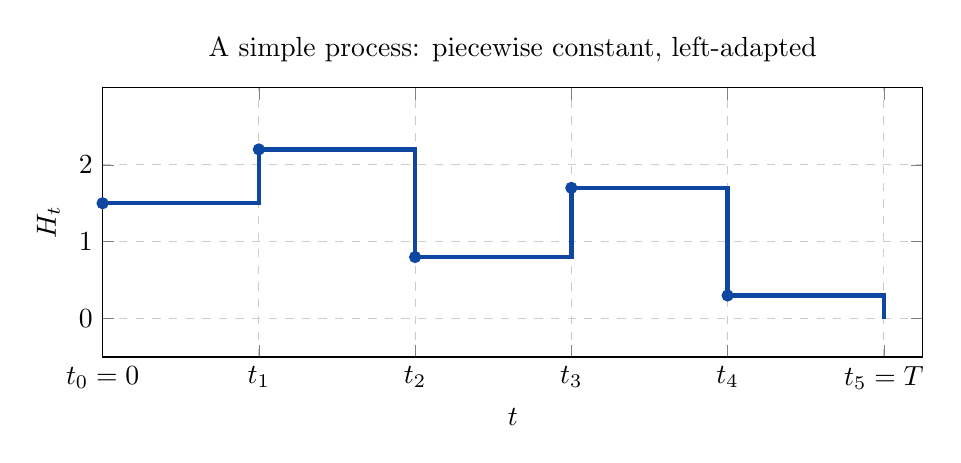
\begin{tikzpicture}
\begin{axis}[
  width=12cm, height=5cm,
  xlabel={$t$}, ylabel={$H_t$},
  xmin=0, xmax=1.05,
  ymin=-0.5, ymax=3,
  xtick={0, 0.2, 0.4, 0.6, 0.8, 1.0},
  xticklabels={$t_0=0$,$t_1$,$t_2$,$t_3$,$t_4$,$t_5=T$},
  ytick={0,1,2},
  grid=major,
  grid style={dashed, gray!40},
  title={A simple process: piecewise constant, left-adapted},
]
\addplot[tutorblue, ultra thick, const plot mark left]
  coordinates {(0,1.5)(0.2,2.2)(0.4,0.8)(0.6,1.7)(0.8,0.3)(1.0,0)};
\foreach \x in {0,0.2,0.4,0.6,0.8}{
  \addplot[tutorblue, mark=*, mark size=2pt] coordinates {(\x, {
    (\x==0)*1.5 + (\x==0.2)*2.2 + (\x==0.4)*0.8 + (\x==0.6)*1.7 + (\x==0.8)*0.3
  })};
}
\end{axis}
\end{tikzpicture}
\caption{A simple process with $n=5$ sub-intervals. Each step $\xi_i$ is fixed at the left endpoint $t_i$ using $\F_{t_i}$-information. The value at $t_5 = T$ is irrelevant (the indicator is $(t_i, t_{i+1}]$, closed on the right).}
\end{figure}

\subsection{Defining the integral of a simple process}

Since each term in~\eqref{eq:simple} is a basic process, and we want the integral to be linear, there is only one possible definition:

\begin{definition}[Itô integral of a simple process]
\label{def:simple-integral}
For the simple process $H_t = \sum_{i=0}^{n-1} \xi_i\,\mathbf{1}_{(t_i,t_{i+1}]}(t)$, the \textbf{Itô integral} is:
\begin{equation}
  \label{eq:simple-integral}
  I(H) = \int_0^T H_t\,dW_t := \sum_{i=0}^{n-1} \xi_i\,(W_{t_{i+1}} - W_{t_i}).
\end{equation}
\end{definition}

\begin{keyidea}
\textbf{This is a weighted sum of Brownian increments.}
Compare equation~\eqref{eq:simple-integral} to the Riemann--Stieltjes sum:
\[
  \sum_{i=0}^{n-1} H(t_i^*)\,(W_{t_{i+1}} - W_{t_i}).
\]
The Itô integral corresponds to always evaluating $H$ at the \emph{left} endpoint $t_i^*= t_i$ of each interval. The critical difference from the Riemann--Stieltjes setting is that $\xi_i = H_{t_i}$ is \emph{random} (not deterministic), and $\xi_i$ must be $\F_{t_i}$-measurable (known at the start of the interval, not at the end). Left-endpoint evaluation is not a convention — it is forced by the requirement of non-anticipatingness.
\end{keyidea}

\subsection{The Itô isometry for simple processes}

All four properties from Proposition~\ref{prop:basic-props} carry over.

\begin{proposition}[Itô isometry for simple processes]
\label{prop:iso-simple}
Let $H$ be a simple process as in Definition~\ref{def:simple}. Then:
\begin{equation}
  \label{eq:isometry}
  \E\left[\left(\int_0^T H_t\,dW_t\right)^2\right] = \E\left[\int_0^T H_t^2\,dt\right].
\end{equation}
\end{proposition}

\begin{proof}[Proof (the magic of orthogonality)]
Write $I(H) = \sum_{i=0}^{n-1} \xi_i(W_{t_{i+1}} - W_{t_i})$. Squaring and taking expectations:
\[
  \E\left[(I(H))^2\right] = \sum_{i=0}^{n-1}\sum_{j=0}^{n-1} \E\bigl[\xi_i(W_{t_{i+1}}-W_{t_i})\cdot \xi_j(W_{t_{j+1}}-W_{t_j})\bigr].
\]
We claim all cross terms (where $i \neq j$) vanish. Without loss of generality, suppose $i < j$. Then $t_i < t_{i+1} \leq t_j < t_{j+1}$. The increment $W_{t_{j+1}} - W_{t_j}$ is independent of $\F_{t_j}$, and the product $\xi_i(W_{t_{i+1}}-W_{t_i}) \cdot \xi_j$ is $\F_{t_j}$-measurable. Therefore:
\[
  \E\bigl[\xi_i(W_{t_{i+1}}-W_{t_i}) \cdot \xi_j(W_{t_{j+1}}-W_{t_j})\bigr] = \E\bigl[\xi_i(W_{t_{i+1}}-W_{t_i})\xi_j\bigr]\cdot \underbrace{\E[W_{t_{j+1}}-W_{t_j}]}_{=\,0} = 0.
\]
Only the diagonal terms survive:
\[
  \E[(I(H))^2] = \sum_{i=0}^{n-1} \E[\xi_i^2]\cdot(t_{i+1}-t_i) = \E\left[\sum_{i=0}^{n-1} \xi_i^2\,(t_{i+1}-t_i)\right] = \E\left[\int_0^T H_t^2\,dt\right]. \qquad \square
\]
\end{proof}

\begin{tutobox}
\textbf{What is the proof really saying?}
The increments of Brownian motion over non-overlapping intervals are independent and mean-zero. So in the double sum $\sum_i\sum_j$, whenever the two intervals $[t_i, t_{i+1}]$ and $[t_j, t_{j+1}]$ do not overlap ($i \neq j$), the contribution is zero by independence. Only the ``diagonal'' $i = j$ terms survive. This is \emph{exactly} the Pythagorean theorem: the gains from disjoint time periods are ``orthogonal'' in $L^2(\Prob)$, so their total variance is just the sum of individual variances.
\end{tutobox}

\subsection{The process $M_t = \int_0^t H_s\,dW_s$ is a martingale}

For a simple process $H$, define the running integral:
\[
  M_t := \int_0^t H_s\,dW_s = \sum_{i:\,t_{i+1}\leq t} \xi_i(W_{t_{i+1}}-W_{t_i}) + \xi_k(W_t - W_{t_k}),
\]
where $t_k$ is the last partition point before $t$. This process is an $(\F_t)$-martingale.

\begin{proof}[Proof sketch]
For $s \leq t$, we want $\E[M_t \mid \F_s] = M_s$. The contribution to $M_t - M_s$ comes from the increments of $W$ after time $s$. These future increments are independent of $\F_s$ and have mean zero. Since each $\xi_i$ is $\F_{t_i}$-measurable and $t_i \geq s$... the detailed proof uses the tower property and independent increments, and goes through cleanly. The conclusion: stochastic integration is the canonical way to manufacture martingales.
\end{proof}

\subsection{Worked examples for simple processes}

\begin{workedex}
\textbf{Example: Computing a simple integral directly.}

Let $T = 1$, partition $t_0 = 0 < t_1 = 0.5 < t_2 = 1$, and:
\[
  H_t = \begin{cases} 1 & t \in (0, 0.5] \\ W_{0.5} & t \in (0.5, 1] \end{cases}
\]
Here $\xi_0 = 1$ (deterministic, trivially $\F_0$-measurable) and $\xi_1 = W_{0.5}$ ($\F_{0.5}$-measurable — we observe $W_{0.5}$ at time 0.5, then decide to hold $\xi_1 = W_{0.5}$ shares during the second half).

The Itô integral is:
\[
  \int_0^1 H_t\,dW_t = \xi_0(W_{0.5} - W_0) + \xi_1(W_1 - W_{0.5}) = 1 \cdot W_{0.5} + W_{0.5}(W_1 - W_{0.5}).
\]
\textbf{Mean check:} $\E[\int_0^1 H_t\,dW_t] = \E[W_{0.5}] + \E[W_{0.5}]\cdot\E[W_1 - W_{0.5}] = 0 + 0 = 0$. \checkmark

\textbf{Variance via isometry:}
\[
  \E\left[\left(\int_0^1 H_t\,dW_t\right)^2\right] = \E\left[\int_0^1 H_t^2\,dt\right] = \E\left[1^2\cdot 0.5 + W_{0.5}^2 \cdot 0.5\right] = 0.5 + 0.5\E[W_{0.5}^2] = 0.5 + 0.5 \cdot 0.5 = 0.75.
\]
\end{workedex}

\begin{workedex}
\textbf{Example: Approximating $\int_0^T W_t\,dW_t$ with simple processes.}

The goal is to compute $\int_0^T W_t\,dW_t$. With simple processes and uniform partition $t_i = iT/n$, the approximating sum is:
\[
  I_n = \sum_{i=0}^{n-1} W_{t_i}(W_{t_{i+1}} - W_{t_i}).
\]
Use the algebraic identity $ab = \frac{1}{2}[(a+b)^2 - a^2 - b^2]$ (``telescope trick''):
\begin{align*}
  W_{t_i}(W_{t_{i+1}} - W_{t_i}) &= \tfrac{1}{2}\bigl(W_{t_{i+1}}^2 - W_{t_i}^2\bigr) - \tfrac{1}{2}(W_{t_{i+1}} - W_{t_i})^2.
\end{align*}
Summing over $i$:
\[
  I_n = \tfrac{1}{2}(W_T^2 - W_0^2) - \tfrac{1}{2}\sum_{i=0}^{n-1}(W_{t_{i+1}} - W_{t_i})^2.
\]
As $n \to \infty$, the sum $\sum_i (W_{t_{i+1}} - W_{t_i})^2 \to T$ (quadratic variation). Since $W_0 = 0$:
\[
  \int_0^T W_t\,dW_t = \frac{W_T^2}{2} - \frac{T}{2}.
\]
\textbf{Compare to classical calculus!} If $f$ were a differentiable function with $f(0)=0$, then $\int_0^T f(t)f'(t)\,dt = \frac{1}{2}f(T)^2$. The Itô result has an extra $-\frac{T}{2}$ correction, which comes from the quadratic variation (i.e., from the $(dW)^2 = dt$ term). This is the hallmark of Itô's formula.
\end{workedex}

% ============================================================
\section{Layer 3: The It\^{o} Integral for Predictable Processes}
\label{sec:predictable}
% ============================================================

So far we can only integrate step functions. Real applications — think of geometric Brownian motion, Black--Scholes delta hedging, or stochastic volatility models — require integrating processes like $H_t = e^{W_t}$ or $H_t = \sigma(t, W_t)$. These are not step functions. We need to extend.

\subsection{The strategy: approximate, integrate, take limits}

The key idea is a standard trick in analysis: if you cannot define a concept for a complicated object directly, find a sequence of simple objects that approximate it, define the concept for each simple object, and show the sequence of results converges.

\begin{tutobox}
\textbf{Analogy with Lebesgue integration.}
Recall how the Lebesgue integral is constructed. You want to integrate a complicated measurable function $f$. You:
\begin{enumerate}
  \item Approximate $f$ by simple functions $f_n$ (finite linear combinations of indicators).
  \item Define $\int f_n$ for each simple function (it is a finite sum).
  \item Show $\int f_n$ converges to a limit $\int f$, independently of the choice of approximating sequence.
\end{enumerate}
The Itô integral follows the exact same blueprint. The approximating objects are simple processes; the norm in which convergence is checked is the $\calL^2$ norm $\norm{\cdot}_{\calL^2}$; and the isometry is what makes the limit well-defined.
\end{tutobox}

\subsection{The class of admissible integrands}

\begin{definition}[The class \texorpdfstring{$\calL^2$}{L2}]
\label{def:L2}
The \textbf{class of admissible integrands} for the Itô integral is:
\[
  \calL^2 = \calL^2([0,T]\times\Omega) = \left\{H : [0,T]\times\Omega\to\R \;\Big|\; H \text{ is predictable and } \E\left[\int_0^T H_t^2\,dt\right] < \infty\right\}.
\]
\end{definition}

\begin{example}
Which processes are in $\calL^2$?
\begin{itemize}
  \item Any bounded predictable process, e.g.\ a simple process.
  \item $H_t = W_t$ (Brownian motion itself): $\E[\int_0^T W_t^2\,dt] = \int_0^T \E[W_t^2]\,dt = \int_0^T t\,dt = T^2/2 < \infty$. \checkmark
  \item $H_t = e^{W_t}$: $\E[e^{2W_t}] = e^{2t}$ (since $e^{W_t}$ is lognormal), so $\E[\int_0^T e^{2W_t}\,dt] = \int_0^T e^{2t}\,dt = \frac{e^{2T}-1}{2} < \infty$. \checkmark
  \item $H_t = e^{W_t^2}$: much larger, but still in $\calL^2$ for finite $T$. \checkmark
\end{itemize}
\end{example}

\subsection{Density of simple processes in \texorpdfstring{$\calL^2$}{L2}}

The following is the key approximation theorem:

\begin{theorem}[Simple processes are dense]
\label{thm:density}
For every $H \in \calL^2$, there exists a sequence of simple processes $(H^{(n)})_{n \geq 1}$ such that:
\[
  \lim_{n\to\infty} \norm{H - H^{(n)}}_{\calL^2}^2 = \lim_{n\to\infty} \E\left[\int_0^T (H_t - H_t^{(n)})^2\,dt\right] = 0.
\]
\end{theorem}

\begin{tutobox}
\textbf{Constructing the approximating sequence.}
For a predictable process $H \in \calL^2$, the most natural approximation is:
\[
  H_t^{(n)} = \sum_{i=0}^{n-1} H_{t_i}\cdot\mathbf{1}_{(t_i,t_{i+1}]}(t), \qquad t_i = \frac{iT}{n}.
\]
This takes the value of $H$ at the left endpoint of each sub-interval and holds it constant. This is well-defined because $H_{t_i}$ is $\F_{t_i}$-measurable (since $H$ is predictable/adapted), and $H^{(n)}$ is a simple process.

Why does $H^{(n)} \to H$ in $\calL^2$? Intuitively: as $n \to \infty$, the sub-intervals shrink to zero, and if $H$ is ``reasonably smooth in time'' (e.g., continuous or left-continuous), then $H^{(n)}_t \approx H_t$ for fine partitions. The formal proof uses the dominated convergence theorem together with the predictability of $H$.

This is completely analogous to approximating a Lebesgue-integrable function by simple functions.
\end{tutobox}

\subsection{The extension theorem}

\begin{theorem}[Itô integral for predictable $L^2$ processes]
\label{thm:main-extension}
For any $H \in \calL^2$, let $(H^{(n)})$ be any sequence of simple processes with $\norm{H - H^{(n)}}_{\calL^2} \to 0$. Then:
\begin{enumerate}[label=(\roman*)]
  \item The sequence $\left(I(H^{(n)})\right)_{n\geq 1} = \left(\int_0^T H_t^{(n)}\,dW_t\right)_{n\geq 1}$ is a Cauchy sequence in $L^2(\Omega, \F, \Prob)$.
  \item The limit $I(H) = \lim_{n\to\infty} I(H^{(n)})$ exists in $L^2$ and is independent of the choice of approximating sequence.
  \item The limit satisfies the \textbf{Itô isometry}:
  \[
    \E\left[\left(\int_0^T H_t\,dW_t\right)^2\right] = \E\left[\int_0^T H_t^2\,dt\right].
  \]
\end{enumerate}
\end{theorem}

\begin{proof}[Proof (step by step)]
\textbf{(i) Cauchy sequence.}
For two simple processes $H^{(n)}, H^{(m)}$, by linearity and the isometry for simple processes:
\[
  \E\left[\left(I(H^{(n)}) - I(H^{(m)})\right)^2\right] = \E\left[\left(I(H^{(n)} - H^{(m)})\right)^2\right] = \E\left[\int_0^T (H_t^{(n)} - H_t^{(m)})^2\,dt\right].
\]
Since $(H^{(n)})$ is Cauchy in $\calL^2$ (because it converges to $H$ in $\calL^2$), the right side goes to zero as $n, m \to \infty$. So $(I(H^{(n)}))$ is Cauchy in $L^2(\Prob)$.

\textbf{(ii) Completeness of $L^2$.}
Every Cauchy sequence in $L^2(\Omega, \F, \Prob)$ converges (this is a classical result: $L^2$ is a complete metric space, i.e., a Hilbert space). So $I(H) = \lim I(H^{(n)})$ exists. Independence of the approximating sequence follows from the same calculation: if $\tilde{H}^{(n)}$ is another sequence with the same limit $H$ in $\calL^2$, then $\E[(I(H^{(n)}) - I(\tilde{H}^{(n)}))^2] = \norm{H^{(n)} - \tilde{H}^{(n)}}_{\calL^2}^2 \to 0$.

\textbf{(iii) Isometry.}
Take the limit $n \to \infty$ in $\E[(I(H^{(n)}))^2] = \norm{H^{(n)}}_{\calL^2}^2$ (which holds for each $n$ by Proposition~\ref{prop:iso-simple}). Both sides converge to the respective limits, giving the isometry for $H$. $\square$
\end{proof}

\begin{tutobox}
\textbf{What the extension theorem is really saying.}
The Itô integral is the unique continuous linear map from $\calL^2$ to $L^2(\Omega)$ that agrees with the simple sum formula on simple processes. This is the same way the Lebesgue integral is the unique continuous extension of the Riemann integral to $L^1$ functions. The isometry is the ``continuity'' of this extension in exactly the sense that matters.

The moral: you never need to explicitly compute the limit of approximating sums in practice. The extension theorem guarantees the integral exists and behaves well. You then use Itô's formula (Section~\ref{sec:ito-formula}) to actually calculate it.
\end{tutobox}

\subsection{Properties of the general Itô integral}

\begin{theorem}[Properties of the Itô integral]
\label{thm:properties}
Let $H, G \in \calL^2$ and $\alpha, \beta \in \R$. Then:
\begin{enumerate}[label=(\roman*)]
  \item \textbf{Linearity}: $\int_0^T (\alpha H_t + \beta G_t)\,dW_t = \alpha\int_0^T H_t\,dW_t + \beta\int_0^T G_t\,dW_t$.
  \item \textbf{Zero mean}: $\E\left[\int_0^T H_t\,dW_t\right] = 0$.
  \item \textbf{Itô isometry}: $\E\left[\left(\int_0^T H_t\,dW_t\right)^2\right] = \E\left[\int_0^T H_t^2\,dt\right]$.
  \item \textbf{Martingale property}: The process $M_t = \int_0^t H_s\,dW_s$ is a continuous square-integrable $(\F_t)$-martingale.
  \item \textbf{Locality}: If $H = G$ a.e.\ on $[0,T]\times\Omega$ (in $\calL^2$-norm), then $I(H) = I(G)$ a.s.
  \item \textbf{Quadratic variation}: $[M]_t = \int_0^t H_s^2\,ds$.
\end{enumerate}
\end{theorem}

Property (iv) deserves extra attention: the martingale property says that Itô integration is the canonical machine for constructing martingales. Property (vi) says that the ``realized variance'' of the integral process is just the $\calL^2$ norm of $H$ up to time $t$.

\subsection{A deeper look: why predictability, not just adaptedness?}

You might ask: why do we need $H$ to be \emph{predictable} rather than merely \emph{adapted}? Isn't adaptedness ($H_t$ is $\F_t$-measurable) sufficient?

For processes with continuous paths, the two notions coincide: every left-continuous adapted process is predictable, and every right-continuous adapted process that is also left-continuous is predictable. For Brownian motion, since $W$ has continuous paths, its natural filtration satisfies $\F_{t^-} = \F_t$, so the distinction disappears.

However, in general:
\begin{itemize}
  \item An adapted process that ``looks at $t$ using future information'' (e.g.\ $H_t = W_{t+\epsilon}$ for some $\epsilon > 0$) is measurable with respect to a $\sigma$-algebra that contains the future, violating non-anticipatingness.
  \item The Itô integral of a non-predictable process loses the martingale property and can have a non-zero drift.
\end{itemize}

In continuous-time finance, predictability is the mathematical formalization of the economic constraint that portfolio strategies cannot anticipate future prices. For right-continuous-with-left-limits (RCLL, or \emph{càdlàg}) filtrations, predictability is equivalent to left-continuity (or measurability w.r.t.\ $\F_{t^-}$).

% ============================================================
\section{The Three Layers: A Side-by-Side Summary}
\label{sec:summary-table}
% ============================================================

\begin{center}
\renewcommand{\arraystretch}{1.6}
\begin{tabular}{@{}llll@{}}
\toprule
& \textbf{Basic} & \textbf{Simple} & \textbf{Predictable} ($\calL^2$) \\
\midrule
\textbf{Form of $H_t$} & $\xi\cdot\mathbf{1}_{(a,b]}(t)$ & $\sum_i \xi_i\mathbf{1}_{(t_i,t_{i+1}]}$ & Any predictable $H$ \\
\textbf{Measurability} & $\xi$ is $\F_a$-meas. & $\xi_i$ is $\F_{t_i}$-meas. & $H_t$ is $\F_{t^-}$-meas. \\
\textbf{Integral formula} & $\xi(W_b - W_a)$ & $\sum_i \xi_i(W_{t_{i+1}}-W_{t_i})$ & Limit of simple integrals \\
\textbf{Definition method} & Direct & Linearity & $L^2$ closure/extension \\
\textbf{Zero mean?} & \checkmark & \checkmark & \checkmark \\
\textbf{Itô isometry?} & \checkmark & \checkmark & \checkmark \\
\textbf{Martingale?} & \checkmark & \checkmark & \checkmark \\
\bottomrule
\end{tabular}
\end{center}

\begin{keyidea}
\textbf{The three layers are a telescope, not three separate theories.}
Basic processes $\subset$ Simple processes $\subset$ Predictable $\calL^2$ processes. Each layer is defined by extending the previous one. The magic is that \emph{all three layers satisfy identical properties}: zero mean, isometry, and martingale. This is because the extension preserves all these properties by continuity ($L^2$ limits preserve $L^2$-closeness, and hence preserve isometries and martingale expectations).
\end{keyidea}

% ============================================================
\section{Itô's Formula: The Payoff of the Theory}
\label{sec:ito-formula}
% ============================================================

Having built the Itô integral, we can state the crowning theorem of the subject. Itô's formula is to stochastic calculus what the chain rule is to ordinary calculus — and as we saw in the $\int W\,dW$ example, it has a correction term that the classical chain rule does not.

\subsection{Itô's formula for Brownian motion}

\begin{theorem}[Itô's formula for $f(W_t)$]
\label{thm:ito-scalar}
Let $f: \R \to \R$ be twice continuously differentiable ($f \in C^2$). Then:
\begin{equation}
  \label{eq:ito-scalar}
  f(W_t) = f(W_0) + \int_0^t f'(W_s)\,dW_s + \frac{1}{2}\int_0^t f''(W_s)\,ds.
\end{equation}
In differential notation:
\[
  df(W_t) = f'(W_t)\,dW_t + \frac{1}{2}f''(W_t)\,dt.
\]
\end{theorem}

\begin{tutobox}
\textbf{Where does the $\frac{1}{2}f''$ term come from?}
Apply the Taylor expansion to $f(W_{t_{i+1}}) - f(W_{t_i})$:
\[
  f(W_{t_{i+1}}) - f(W_{t_i}) = f'(W_{t_i})(W_{t_{i+1}}-W_{t_i}) + \frac{1}{2}f''(W_{t_i})(W_{t_{i+1}}-W_{t_i})^2 + O(\abs{\Delta W_i}^3).
\]
Sum over $i$: the first sum gives the Itô integral $\int f'(W)\,dW$. The second sum involves $(W_{t_{i+1}} - W_{t_i})^2$, and by Proposition~\ref{prop:qv}, this converges to $\int_0^t dt = t$ (quadratic variation). In classical calculus, $(dx)^2 = 0$ so this term would vanish. But for Brownian motion, $(dW)^2 = dt \neq 0$, so the second-order term survives and becomes $\frac{1}{2}\int f''(W_s)\,ds$. This is the Itô correction.
\end{tutobox}

\subsection{General Itô's formula for an Itô process}

In most applications, the integrator is not just $W_t$ but an \emph{Itô process}:
\[
  dX_t = \mu_t\,dt + \sigma_t\,dW_t,
\]
where $\mu_t$ is an adapted drift and $\sigma_t \in \calL^2$ is an adapted diffusion coefficient.

\begin{theorem}[General Itô's formula]
\label{thm:ito-general}
Let $X_t$ be an Itô process with $dX_t = \mu_t\,dt + \sigma_t\,dW_t$, and let $f(t,x) \in C^{1,2}$ (once continuously differentiable in $t$, twice in $x$). Then:
\begin{equation}
  \label{eq:ito-general}
  df(t, X_t) = \frac{\partial f}{\partial t}\,dt + \frac{\partial f}{\partial x}\,dX_t + \frac{1}{2}\frac{\partial^2 f}{\partial x^2}\,(dX_t)^2,
\end{equation}
where $(dX_t)^2$ is computed using the Itô multiplication table: $(dt)^2 = 0$, $dt\,dW_t = 0$, $(dW_t)^2 = dt$. Expanding:
\[
  df(t, X_t) = \left(\frac{\partial f}{\partial t} + \mu_t\frac{\partial f}{\partial x} + \frac{\sigma_t^2}{2}\frac{\partial^2 f}{\partial x^2}\right)dt + \sigma_t\frac{\partial f}{\partial x}\,dW_t.
\]
\end{theorem}

\begin{workedex}
\textbf{Deriving geometric Brownian motion.}
Let $X_t = \mu t + \sigma W_t$ (arithmetic Brownian motion with drift). We want to find $S_t = e^{X_t}$.

Let $f(t,x) = e^x$ (no explicit $t$ dependence). Then $f' = f'' = e^x$. Itô's formula gives:
\[
  dS_t = de^{X_t} = e^{X_t}\,dX_t + \frac{1}{2}e^{X_t}(dX_t)^2 = S_t(\mu\,dt + \sigma\,dW_t) + \frac{1}{2}S_t\sigma^2\,dt.
\]
Collecting:
\[
  dS_t = S_t\left(\mu + \frac{\sigma^2}{2}\right)dt + S_t\sigma\,dW_t.
\]
This is the Black--Scholes SDE for a stock price. The drift of $S_t$ is $\mu + \frac{\sigma^2}{2}$, not just $\mu$. The extra $\frac{\sigma^2}{2}$ is the Itô correction — it represents the compounding benefit of the volatility. This is also why the lognormal distribution for returns has mean $(\mu + \sigma^2/2)t$, not $\mu t$.
\end{workedex}

\begin{workedex}
\textbf{Recovering $\int_0^T W_t\,dW_t = \frac{1}{2}W_T^2 - \frac{T}{2}$.}

Apply Itô's formula to $f(x) = x^2/2$, so $f'(x) = x$ and $f''(x) = 1$:
\[
  \frac{1}{2}W_T^2 - \frac{1}{2}W_0^2 = \int_0^T W_t\,dW_t + \frac{1}{2}\int_0^T 1\,dt.
\]
Since $W_0 = 0$:
\[
  \int_0^T W_t\,dW_t = \frac{1}{2}W_T^2 - \frac{T}{2}.
\]
The Itô term $-T/2$ is exactly the correction from $(dW)^2 = dt$. Classical calculus (with $f(x) = x^2/2$, $f'(x) = x$, $df/dx = x$) would give $\int_0^T x\,dx = x^2/2|_0^T = T^2/2$, which is completely different. Brownian motion is not a classical function; its ``self-integral'' feels the quadratic variation.
\end{workedex}

% ============================================================
\section{The Martingale Representation Theorem (A Taste)}
\label{sec:mrt}
% ============================================================

We close with a deep theorem that illustrates the power of the integral we have built.

\begin{theorem}[Martingale Representation Theorem, MRT]
Let $(M_t)_{t \in [0,T]}$ be a continuous square-integrable martingale with respect to the filtration generated by $W$. Then there exists a unique predictable process $H \in \calL^2$ such that:
\[
  M_t = M_0 + \int_0^t H_s\,dW_s, \qquad \text{a.s. for all } t \in [0,T].
\]
\end{theorem}

\begin{tutobox}
\textbf{What MRT is saying.}
Every martingale (with respect to a Brownian filtration) is an Itô integral. This is a remarkable statement: it says that the only way to build a martingale in a Brownian-motion world is through stochastic integration. There is no other martingale. This theorem is the heart of complete-market financial theory: in a Black--Scholes world, every contingent claim (option payoff) can be replicated by a trading strategy (a process $H_t$), because every payoff that has the martingale structure (under the risk-neutral measure) is representable as a stochastic integral.
\end{tutobox}

% ============================================================
\section{Putting It All Together: A Road Map}
\label{sec:roadmap}
% ============================================================

\begin{tutobox}
\textbf{The logical arc, in one paragraph.}
Classical integrals ($\int f\,dt$ and $\int f\,dg$) require the integrator to have finite variation. Brownian motion has infinite variation, so classical integration against $dW$ is undefined. But Brownian increments over non-overlapping intervals are independent and mean-zero, which is a form of \emph{orthogonality}. We exploit this orthogonality in the Itô isometry $\E[(\int H\,dW)^2] = \E[\int H^2\,dt]$. We first define the integral for the simplest integrands (basic processes = single indicator), then for finite sums (simple processes = step functions), proving the isometry at each step using independence of increments. Finally, since simple processes are dense in the Hilbert space $\calL^2$, we extend the integral to all of $\calL^2$ by a completion argument. The extension inherits zero-mean, isometry, and martingale properties. Itô's formula is then derived by Taylor-expanding $f(W_t)$ and recognizing the quadratic variation $(dW)^2 = dt$ as the source of the correction term. Every martingale in a Brownian world is an Itô integral (MRT), which is the mathematical reason complete financial markets can replicate every derivative payoff.
\end{tutobox}

\subsection*{Checklist: Things you should be able to do after reading these notes}

\begin{itemize}[label=$\square$]
  \item Explain in one sentence why the Riemann--Stieltjes integral fails for Brownian motion.
  \item State the definition of a basic process and compute its Itô integral directly.
  \item State the definition of a simple process and compute its Itô integral as a sum.
  \item Prove the Itô isometry for simple processes using the independence-of-increments argument.
  \item Explain (in words, without full proof) why the integral can be extended from simple to $\calL^2$ processes, and what the isometry's role is in that extension.
  \item Identify whether a given process is adapted, predictable, or neither.
  \item Verify that $\int_0^T W_t\,dW_t = \frac{1}{2}W_T^2 - \frac{1}{2}T$ using either the direct sum calculation or Itô's formula.
  \item Apply Itô's formula to find the SDE satisfied by $f(t, X_t)$ given the SDE for $X_t$.
  \item State (not prove) the Martingale Representation Theorem and explain its financial interpretation.
\end{itemize}

% ============================================================
\appendix
\section{Appendix: The Itô Multiplication Table Derived}
\label{app:mult-table}
% ============================================================

The informal rules $(dW)^2 = dt$, $dW\cdot dt = 0$, $(dt)^2 = 0$ can be made rigorous as follows.

Let $\Pi_n$ be a partition of $[0,T]$ with mesh $\abs{\Pi_n} \to 0$.

\textbf{$(dW)^2 = dt$:} The quadratic variation result (Proposition~\ref{prop:qv}) states:
\[
  \sum_{i} (W_{t_{i+1}} - W_{t_i})^2 \xrightarrow{L^2} T.
\]
For a general test function $f(t)$:
\[
  \sum_{i} f(t_i)(W_{t_{i+1}}-W_{t_i})^2 \xrightarrow{L^2} \int_0^T f(t)\,dt,
\]
which is written $\int_0^T f(t)(dW_t)^2 = \int_0^T f(t)\,dt$, i.e.\ $(dW_t)^2 = dt$.

\textbf{$dW \cdot dt = 0$:}
\[
  \sum_{i}(W_{t_{i+1}}-W_{t_i})(t_{i+1}-t_i) \leq \max_i(t_{i+1}-t_i)\cdot \sum_i\abs{W_{t_{i+1}}-W_{t_i}}.
\]
In $L^2$, $\max_i(t_{i+1}-t_i) \to 0$ and $\sum_i\abs{W_{t_{i+1}}-W_{t_i}}$ is bounded in $L^2$ (by arguments involving Doob's inequality), so the product $\to 0$.

\textbf{$(dt)^2 = 0$:}
\[
  \sum_i (t_{i+1}-t_i)^2 \leq \abs{\Pi_n}\cdot\sum_i(t_{i+1}-t_i) = \abs{\Pi_n}\cdot T \to 0.
\]

% ============================================================
\section{Appendix: Proof of the Quadratic Variation of Brownian Motion}
\label{app:qv}
% ============================================================

We prove Proposition~\ref{prop:qv}: for a uniform partition $t_i = iT/n$,
\[
  Q_n = \sum_{i=0}^{n-1}(W_{t_{i+1}}-W_{t_i})^2 \xrightarrow{L^2} T.
\]

Let $\Delta_i = W_{t_{i+1}} - W_{t_i} \sim \mathcal{N}(0, T/n)$. Then:
\[
  \E[Q_n] = \sum_{i=0}^{n-1}\E[\Delta_i^2] = n \cdot \frac{T}{n} = T.
\]
\[
  \var(Q_n) = \sum_{i=0}^{n-1}\var(\Delta_i^2) = n\cdot\var(\Delta_i^2).
\]
For $X \sim \mathcal{N}(0,\sigma^2)$: $\var(X^2) = \E[X^4] - (\E[X^2])^2 = 3\sigma^4 - \sigma^4 = 2\sigma^4$.
Here $\sigma^2 = T/n$, so $\var(\Delta_i^2) = 2(T/n)^2$, and:
\[
  \var(Q_n) = n\cdot 2\left(\frac{T}{n}\right)^2 = \frac{2T^2}{n} \to 0.
\]
Since $\E[Q_n] = T$ and $\var(Q_n) \to 0$, we have $Q_n \xrightarrow{L^2} T$. $\square$

% ============================================================
\section{Appendix: Commonly Used Results at a Glance}
\label{app:ref}
% ============================================================

\begin{center}
\renewcommand{\arraystretch}{2.0}
\begin{tabular}{@{}ll@{}}
\toprule
\textbf{Result} & \textbf{Formula} \\
\midrule
BM increment distribution & $W_t - W_s \sim \mathcal{N}(0, t-s)$ \\
Quadratic variation & $\sum_i(W_{t_{i+1}}-W_{t_i})^2 \xrightarrow{L^2} T$ \\
Itô integral (simple) & $\displaystyle\int_0^T H_t\,dW_t = \sum_{i=0}^{n-1}\xi_i(W_{t_{i+1}}-W_{t_i})$ \\
Zero mean & $\displaystyle\E\left[\int_0^T H_t\,dW_t\right] = 0$ \\
Itô isometry & $\displaystyle\E\!\left[\!\left(\int_0^T H_t\,dW_t\right)^2\right] = \E\!\left[\int_0^T H_t^2\,dt\right]$ \\
Itô's formula & $\displaystyle df(t,X_t) = f_t\,dt + f_x\,dX_t + \tfrac{1}{2}f_{xx}(dX_t)^2$ \\
Mult.\ table & $(dW)^2 = dt$,\; $dW\cdot dt = 0$,\; $(dt)^2 = 0$ \\
Key example & $\displaystyle\int_0^T W_t\,dW_t = \tfrac{1}{2}W_T^2 - \tfrac{T}{2}$ \\
GBM SDE & $dS_t = \mu S_t\,dt + \sigma S_t\,dW_t \Rightarrow S_t = S_0\,e^{(\mu-\sigma^2/2)t+\sigma W_t}$ \\
MRT & Every BM-filtration martingale $=$ an Itô integral \\
\bottomrule
\end{tabular}
\end{center}

\vspace{2em}
\hrule height 1pt
\vspace{1em}
{\small\textit{These notes are written for pedagogical clarity. Proofs are complete where the proof itself is instructive; otherwise, a rigorous sketch and reference is provided. All results are standard and can be found in Øksendal (2003), Shreve (2004), or Protter (2005).}}

\end{document}
